\begin{frame}{Motivation}

\begin{itemize}
\itemsep1pt\parskip0pt\parsep0pt
\item
  Test correctness of later compiled implementations
\item
  Fully implement non-determinacy
\item
  Familiarise language implementers with the semantics of GP 2
\item
  Identify any gaps or ambiguities in the semantics
\end{itemize}

\pause

\textbf{Simplicity is an over-riding aim}

\begin{itemize}
\itemsep1pt\parskip0pt\parsep0pt
\item
  Speed and memory use are secondary concerns
\item
  Sophistication is to be actively avoided if it complicates the
  implementation!
\end{itemize}

\end{frame}

\begin{frame}{Requirements 1}

General requirements:

\begin{itemize}
\itemsep1pt\parskip0pt\parsep0pt
\item
  Quick to develop 
\item
  Easy to maintain and reason about
\item
  Must be fast enough to do ``useful work''
\end{itemize}

\pause

For a given program/host-graph pair\ldots{}

\begin{itemize}
\itemsep1pt\parskip0pt\parsep0pt
\item
  Generate all possible output graphs 
\item
  Produce all distinct output graphs up to isomorphism 
\item
  Output a single result 
\end{itemize}

\end{frame}

\begin{frame}{Requirements 2}

Also, stand-alone tools:

\begin{itemize}
\itemsep1pt\parskip0pt\parsep0pt
\item
  Isomorphism checker
\item
  Host-graph generator
\item
  Graph viewer
\end{itemize}

\end{frame}

\begin{frame}{Implementation 1}

\begin{itemize}
\itemsep1pt\parskip0pt\parsep0pt
\item
  Based on the GP 2 semantics
\item
  Written in Haskell\footnote{\url{https://www.haskell.org/}}
\end{itemize}

\begin{center}
\scalebox{0.9}{ \begin{tikzpicture} [align=center, arrowout]

\node(parser) at (0,0)  [box, rounded corners] {Parser};

\node(gen) at (3,0) [box, rounded corners] {Transformer};

\node(inter) at (6.5,0) [box, rounded corners] {Interpreter};

\node(apply) at (4.5,-2) [box, rounded corners] {Rule Applier};

\draw[arrowout] (-2, 0.22) -- node[above, text width=1.5cm]{\scriptsize{Host Graph File}} (parser.160);
\draw[arrowout] (-2, -0.22) -- node[below, text width=1.5cm]{\scriptsize{Program File}} (parser.200);
\draw[arrowout] (0,-1.7) -- node[right, text width=1.5cm]{\scriptsize{Rule Application Bound}} (parser.270);

\draw [arrowout] (parser) --  (gen);
\node at (1.35,0.3) {\scriptsize{AST}};

\draw [arrowout] (gen.10) -- node[above, text width=1cm]{\scriptsize{Host Graph}} (inter.167);
\draw [arrowout] (gen.350) --  (inter.193);
\node at (4.9,-0.5) [text width=1cm]{\scriptsize{Program}};

\draw [arrowout] (inter.325) |- (apply.350);
\node at (7.8,-1.3) {\scriptsize{Rule}};

\draw [arrowout] (inter.310) |- (apply.10);
\node at (6.4, -1.3) [text width=1cm]{\scriptsize{Host Graph}};

\draw [arrowout] (apply.90) --  (inter.225);
\node at (4.6,-1) {\scriptsize{Graphs}};

\draw[arrowout] (inter) -- node[above, text width=1cm]{\scriptsize{Output Data}} (8.5,0);

\end{tikzpicture}


 }
\end{center}

\end{frame}

\begin{frame}{Implementation 2}

\begin{center}
\small
\scalebox{0.65}{\begin{tikzpicture} [align=center]

\node(main) at (0, 0)  [box] {Main\\Interpreter\\53 lines};
\node(iso) at (2.5, -2.25) [box] {Isomorphism\\Checker\\21 lines};
\node(print) at (2.5, -0.75) [box] {Graph Printer\\34 lines};
\node(eval) at (2.5, 0.75) [box] {Evaluator\\99 lines};
\node(parser) at (2.5, 2.25) [box] {Parser\\230 lines};
\node(apply) at (5, 0.75) [box] {Rule\\Applier\\53 lines};
\node(gmatch) at (7.5, 0.75) [box] {Graph\\Matcher\\43 lines};
\node(graph) at (7.5, -1.5) [box] {Graph\\Library\\76 lines};
\node(lmatch) at (10, -1.5) [box] {Label\\Matcher\\89 lines};
\node(trans) at (10, 0.75) [box] {Checker \&\\Transformer\\118 lines};
\node(libs) at (12.5, -1.5) [box] {Lists \&\\Finite Maps\\60 lines};
\node(ast) at (12.5, 0.75) [box] {AST\\126 lines};

\draw (ast) edge[arrowin, dashed] (trans);
\draw (ast) edge[arrowin, dashed] (lmatch);
\draw (ast.145) edge[arrowin, dashed, bend right=15] (parser);
\draw (libs) edge[arrowin, dashed] (trans);
\draw (libs) edge[arrowin, dashed] (lmatch);
\draw (libs.215) edge[arrowin, dashed, bend left=25] (graph.315);
\draw (trans) edge[arrowin, dashed] (gmatch);
\draw (graph) edge[arrowin, dashed] (gmatch);
\draw (graph) edge[arrowin, dashed] (iso.0);
\draw (graph) edge[arrowin, dashed] (print.0);
\draw (lmatch) edge[arrowin, dashed] (gmatch);
\draw (gmatch.180) edge[arrowin, dashed] (apply);
\draw (apply) edge[arrowin, dashed] (eval.0);
\draw (parser.180) edge[arrowin, dashed] (main);
\draw (iso.180) edge[arrowin, dashed] (main);
\draw (eval.180) edge[arrowin, dashed] (main);
\draw (print.180) edge[arrowin, dashed] (main);

\end{tikzpicture}


}
\end{center}

\begin{itemize}
\itemsep1pt\parskip0pt\parsep0pt
\item
  Approx. 1000 SLOC
\item
  Exploits distinctive features of Haskell to achieve conciseness:

  \begin{itemize}
  \itemsep1pt\parskip0pt\parsep0pt
  \item
    list-comprehensions
  \item
    lazy evaluation
  \end{itemize}
\end{itemize}

\end{frame}

\begin{frame}{Performance}

\begin{itemize}
\itemsep1pt\parskip0pt\parsep0pt
\item
  Produce a fourth-generation Sierpinski triangle in 6.5 seconds 
\item
  A cyclic graph of 1000 nodes fails an acyclicity test in 1.8 seconds 
\item
  Transitive closure of a linear graph of 50 nodes takes 66 seconds
\item
  Vertex colouring a 9x9 grid in one-result mode takes less than a
  second\ldots{}
\item
  \ldots{}but in all-result mode exceeds 5 minutes with only a 3x3 grid 
\end{itemize}

A more detailed discussion of performance can be found in the paper

\end{frame}

\begin{frame}{Conclusions}

\begin{itemize}
\itemsep1pt\parskip0pt\parsep0pt
\item
  We have developed a useful reference tool for our ongoing research
\item
  Also useful ancillary tools:

  \begin{itemize}
  \itemsep1pt\parskip0pt\parsep0pt
  \item
    GraphViz-based graph visualiser
  \item
    Stand-alone isomorphism checker
  \item
    Host-graph generator, based on hypergraph grammars 
  \end{itemize}
\item
  Gained a clear understanding of the GP 2 semantics
\item
  Become aware of some `edge-cases' that might trip us up in our
  compiler work 
\end{itemize}

\end{frame}

\begin{frame}{Further work}

\begin{itemize}
\itemsep1pt\parskip0pt\parsep0pt
\item
  Better error reporting
\item
  A performant compiler 
\item
  GUI program editor
\item
  Formal verification against GP 2 semantics. 
\end{itemize}

\begin{center}
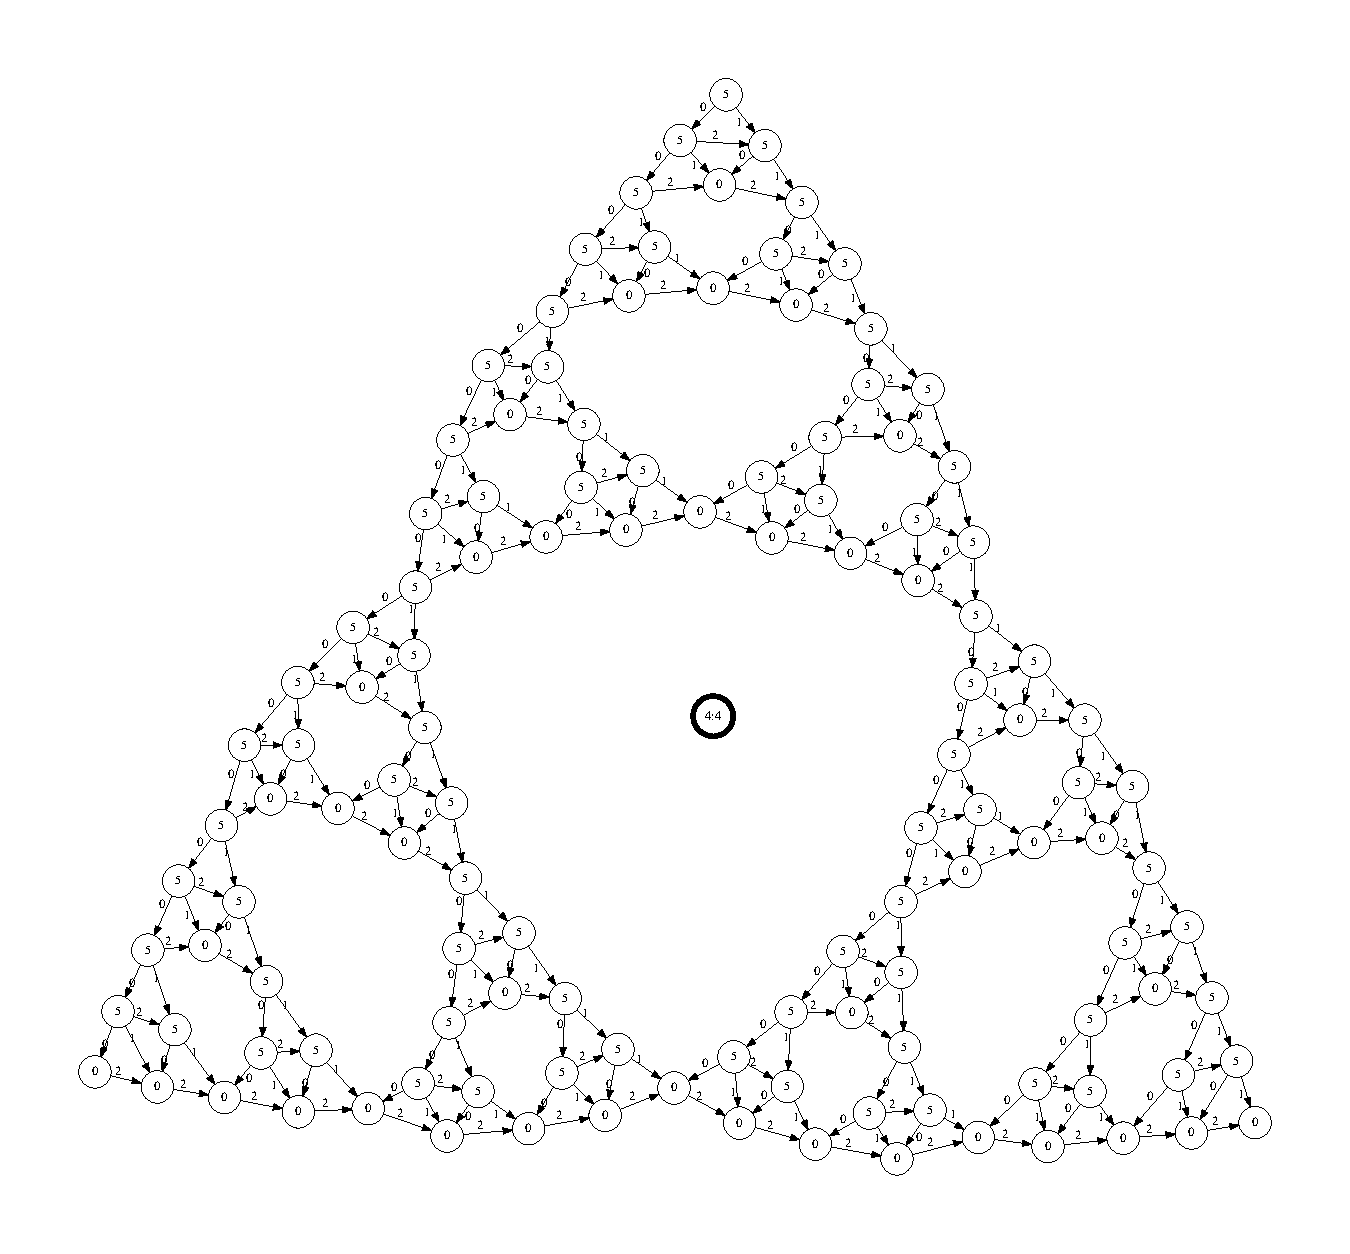
\includegraphics[scale=0.2]{gp2graph_9CRkVV.pdf}
\end{center}

\end{frame}
